\documentclass[conference]{IEEEtran}
\IEEEoverridecommandlockouts
\usepackage{cite}
\usepackage{amsmath,amssymb,amsfonts}
\usepackage{algorithmic}
\usepackage{graphicx}
\usepackage{textcomp}
\usepackage{booktabs}
\usepackage{tabularx}
\usepackage{hyperref}
\usepackage{soul}
\usepackage[dvipsnames]{xcolor}

\begin{document}

\title{Hybrid Cellular-LoRa Network Based Agriculture Monitoring and Control Application for Hobby Gardens without Internet Access}

\author{\IEEEauthorblockN{Yusuf Çağrı Öğüt}
\IEEEauthorblockA{Computer Engineering Department, Hacettepe University, Ankara, Türkiye\\
Student ID: N25240126}}

\maketitle

\begin{abstract}
This project addresses the lack of internet connectivity in hobby gardens by proposing a hybrid communication architecture \cite{enock2025lora}, \cite{heble2018low}, \cite{islam2021performance}, \cite{lorawan2025}. The system combines a Wide Area Network (WAN) using cellular SMS for remote control and a Local Area Network (LAN) utilizing LoRa for communication between sensor and actuator nodes. The architecture includes a central controller, field controllers, moisture \cite{sudan2025}, temperature, and flow sensors, and latched-valve actuators, optimized for low-power operation and powered by a optionally solar-charged battery system. The methodology involves a complete embedded system pipeline from hardware integration to firmware development, with a focus on real-world constraints such as underground deployment and energy efficiency.
\end{abstract}

\begin{IEEEkeywords}
Embedded Systems, LoRa, Cellular Networks, Smart Agriculture, Low-Power Design.
\end{IEEEkeywords}

\section{Introduction}
Many hobby gardens are situated in remote locations where traditional internet connectivity is unavailable. This lack of infrastructure prevents the use of standard IoT solutions for monitoring and irrigation. This project proposes a hybrid network consisting of a cellular-based WAN and a LoRa-based LAN to enable remote monitoring and valve control via SMS. The goal is to provide a robust, cost-friendly, and energy-efficient solution for gardeners who cannot visit their plots daily.

\section{Problem Definition}
Gardeners often face challenges in maintaining irrigation due to limited water availability windows and the distance to hobby gardens. Existing offline solutions lack the robustness to report faults like clogged pipes or valve failures. 

\subsection{Objectives}
The primary objective is to build a remote-controlled irrigation system that operates without internet, providing sensory feedback (moisture, temperature, flow) to the user via SMS.

\subsection{Constraints}
\begin{itemize}
    \item \textbf{Connectivity:} No internet access; must rely on SMS and LoRa.
    \item \textbf{Power:} Must operate autonomously using battery and/or solar power.
    \item \textbf{Environment:} Hardware must withstand underground deployment and environmental factors.
\end{itemize}
One of the biggest challenges in the system is power consumption One of the hardships of the project will be managing power consumption. A
preliminary power budget calculation is done. As microcontroller will be in sleep
mode mostly, it will work 23.9 hours of day, energy consumption will be 0.14mAh
consumptions per day. It is planned that sensors will be checked every 20 minutes.
This corresponds to 0.1mAh per day. For energy efficiency a latched-valve will be
used, which doesn’t require energy for holding it’s position. They generally draw
1 amperes in each work cycle and it takes approximately 50 ms. Considering
closing and opening motions, it will draw 0.03 mAh per day. LoRa is in deep
sleep mode in \%99 of times. Therefore, it has a power consumption of 0.7 mAh
per day. Total consumption corresponds to around 1 mAh per day. Considering
using 10 lines for the system, the total is 30 mAh per day. the battery planned
to be is a standard li-po battery with capacity of 3.000 mAh. This means in ideal
conditions battery will last 100 days without charging. Note that this might be
reduced as battery will be placed under the ground, moisture and cold will drop
it’s performance. Another issue is that for protecting battery health, it’s charge
should be kept around \%80 percent. To ensure that a solar panel and a simple
charging circuit is planned to be used. By these cautions, power will not be a
problem for the system.
\section{System Architecture and Design}
The system architecture is divided into two main domains:
\begin{itemize}
    \item \textbf{WAN:} Includes a remote mobile device and a SIM module serving as the interface to the central controller.
    \item \textbf{LAN:} Consists of a central controller and 2-3 sensor/actuator nodes communicating via LoRa.
\end{itemize}
\begin{figure}[ht!]
    \centering
    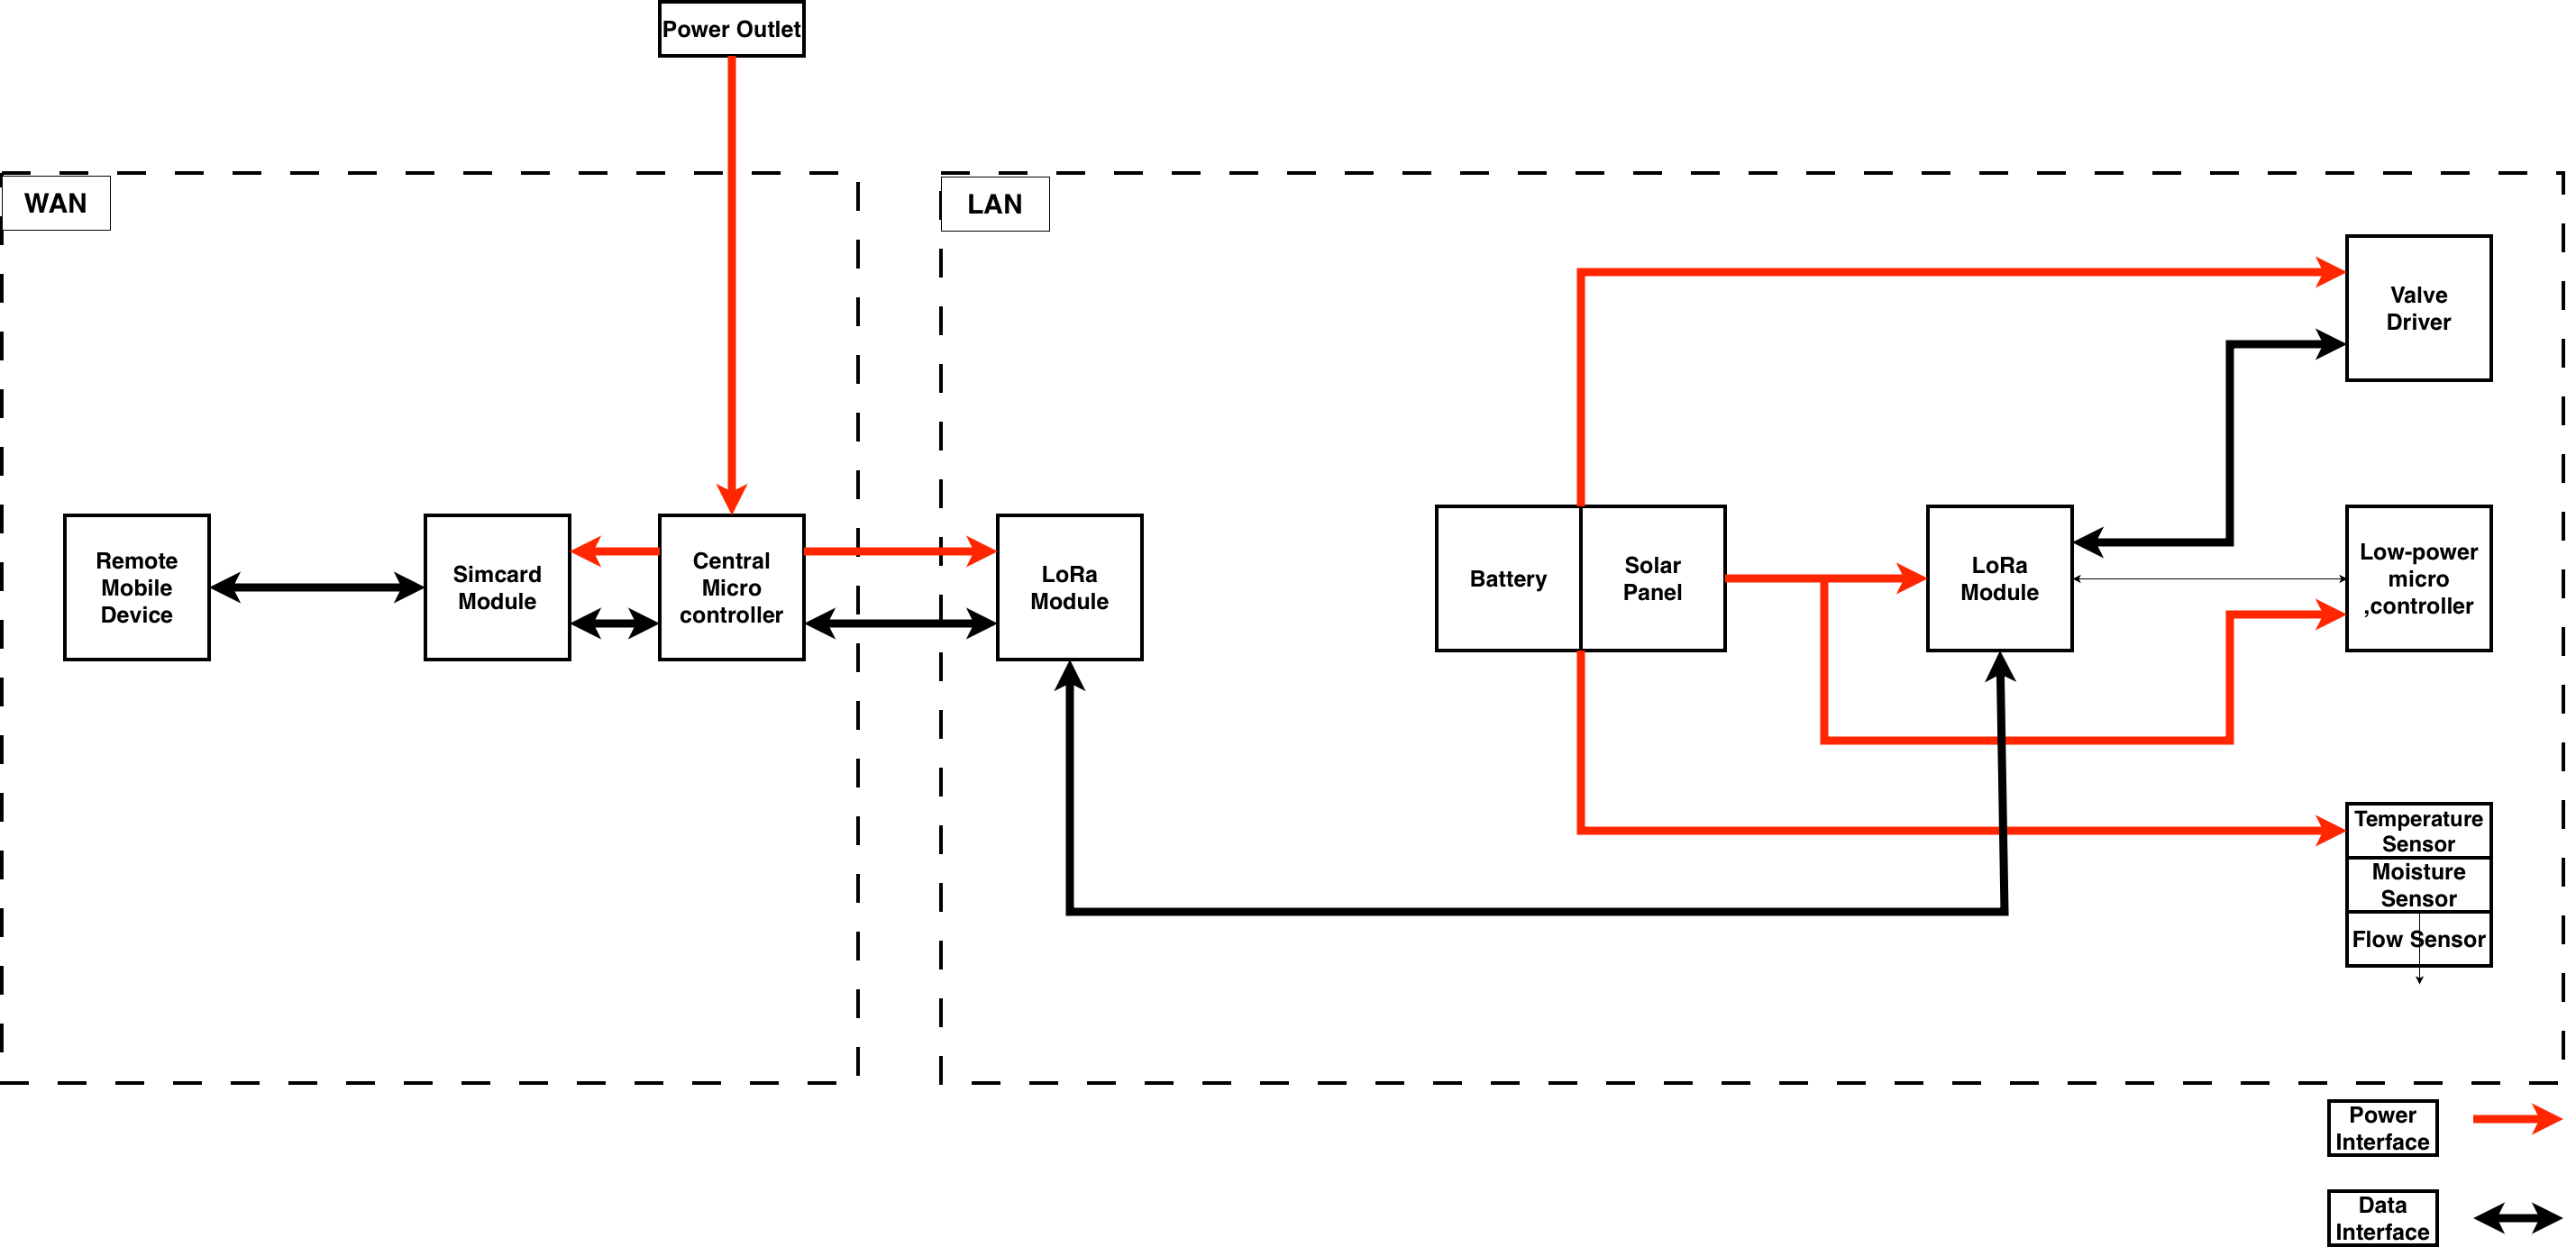
\includegraphics[width=\linewidth]{schematic.png}
    \caption{System architecture}
    \label{fig:smalldiagram}
\end{figure}
\subsection{Hardware Architecture}
The LAN nodes utilize low-power microcontrollers integrated with moisture, temperature, and flow sensors. For actuation, latched-valves are used to minimize energy consumption as they do not require power to maintain their state.

\subsection{Requirements Analysis}\label{sec:reqs}

\subsubsection{Functional Requirements}
\begin{enumerate}
    \item The system shall provide a remote interface via SMS to open/close specific irrigation valves.
    \item The system shall collect and report soil moisture, ambient temperature, and water flow data.
    \item The central controller shall bridge commands between the cellular WAN and the local LoRa sensor/actuator network.
    \item The system shall automatically enter deep-sleep modes between active cycles to maintain the power budget.
    \item The sensor nodes shall perform local data processing before transmission to minimize radio uptime.
\end{enumerate}

\subsubsection{Non-Functional Requirements}
\begin{itemize}
    \item \textbf{Network Scalability:} The local LoRa network shall support at least 2--3 sensor/actuator nodes for the semester prototype, with an architectural capacity for future expansion.
    \item \textbf{Latency:}
    \begin{itemize}
        \item The maximum end-to-end latency for a valve control command ($SMS \rightarrow controller \rightarrow valve$) shall not exceed 60 seconds.
        \item Sensor data reporting latency shall be configured for 20-minute intervals to balance real-time awareness with energy conservation.
    \end{itemize}
    \item \textbf{Reliability and Fault Tolerance:}
    \begin{itemize}
        \item The system shall implement a "Safe State" mechanism where valves close automatically if communication with the central controller is lost for more than 1 hour.
        \item The system shall detect and report sensor hardware failures or signal integrity loss via a status SMS.
    \end{itemize}
    \item \textbf{Security:} The central controller shall only execute commands from a pre-authorized "White-list" of mobile numbers to ensure command validation.
    \item \textbf{Physical Durability:} Buried components shall be housed in IP67-rated enclosures to withstand high moisture and soil pressure\cite{balivada2022wireless}.
    \item \textbf{Physical Durability-2:} Communication modules located outdoors should be kept at least 20 cm high from ground \cite{yu2012research}.
\end{itemize}
\subsection{Communication Protocols and Timing Assumptions}

To ensure reliable operation in environments without internet access while maintaining a strict power budget, the system employs a tiered communication strategy and a synchronized execution model.

\subsubsection{Communication Protocols}
The system bridges two distinct network tiers:
\begin{itemize}
    \item \textbf{WAN Tier (GSM/SMS):} Communication between the user and the Central Controller utilizes standard SMS protocols. A lightweight, text-based command set (e.g., \texttt{V1\_OPEN}, \texttt{STATUS\_REQ}) is used to ensure compatibility with basic cellular modules and minimize transmission costs.
    \item \textbf{LAN Tier (LoRa):} Local communication between the Central Controller and sensor nodes utilizes LoRa modulation. To minimize power consumption, the protocol uses raw binary payloads rather than high-overhead headers, including a Node ID and CRC for packet integrity.
\end{itemize}

\subsubsection{System Timing and Scheduling}
The system's feasibility relies on precise timing assumptions to manage the 1~mAh/day energy goal:
\begin{itemize}
    \item \textbf{Duty Cycle:} All sensor nodes operate on a 99\% deep-sleep duty cycle. Nodes wake up exactly every 20 minutes to sample data and check for pending commands.
    \item \textbf{Active Windows:} Upon waking, each node stays active for a maximum of 5 seconds to perform sensing and radio transmission before returning to sleep.
    \item \textbf{Command Latency:} Based on the 20-minute polling interval, the maximum latency for a non-urgent status report is 20 minutes. However, the end-to-end latency for a high-priority valve command ($SMS \rightarrow controller \rightarrow valve$) is assumed to be under 60 seconds once the controller receives the SMS.
    \item \textbf{Collision Avoidance:} The Central Controller uses a time-slotted approach to poll nodes sequentially, preventing packet collisions in the LoRa frequency band.
\end{itemize}
\section{System-Level Considerations}
\begin{itemize}
    \item \textbf{Energy Efficiency:} Utilization of sleep modes (99\% deep sleep for LoRa) and latched valves to extend battery life to approximately 100 days.
    \item \textbf{Reliability:} Use of shielded cables to maintain signal integrity over distances up to 10 meters and protective coverage for buried components.
    \item \textbf{Security:} SMS command validation will be implemented to prevent unauthorized access.
\end{itemize}

\section{Implementation Plan}
The project will follow these milestones:
\begin{itemize}
    \item \textbf{Phase 1:} Requirement specification and communication architecture definition.
    \item \textbf{Phase 2:} Hardware integration (sensors, LoRa, and cellular modules).
    \item \textbf{Phase 3:} Firmware development and testing of energy consumption assumptions.
    \item \textbf{Phase 4:} Final evaluation and deployment in realistic conditions.
\end{itemize}
\section{Experimental Setup}

This section describes the evaluation environment and the specific metrics used to validate the hybrid communication architecture and power management strategy.

\subsection{Platform and Tools}
The implementation and evaluation will utilize the following hardware and software tools:
\begin{itemize}
    \item \textbf{Microcontrollers:} Low-power stm32 based mcu's for sensor nodes and a central gateway node.
    \item \textbf{Communication Modules:} Ra-02 IPX 433MHz LoRaWAN modules for local networking and a SIM800L module for GSM/SMS connectivity.
    \item \textbf{Development Environment:} STM32CudeIDE and STM32CubeMX for software development and hardware interfacing.
    \item \textbf{Simulation/Analysis:} A digital multimeter and an oscilloscope will be used to profile the current consumption during active, transmit, and deep-sleep states to verify the 1~mAh/day power budget.
\end{itemize}

\subsection{Datasets and Workloads}
As this is a physical implementation, the "workload" consists of real-time environmental data and simulated user interactions:
\begin{itemize}
    \item \textbf{Environmental Data:} Moisture levels ranging from 0\% to 100\% (simulated via soil saturation), temperature fluctuations, and water flow pulses.
    \item \textbf{Control Workload:} A standardized test set of 50 SMS commands sent at varying intervals to measure gateway responsiveness and valve actuation success rates.
\end{itemize}

\subsection{Evaluation Metrics}
The system will be evaluated against the following primary metrics:
\begin{itemize}
    \item \textbf{Communication Latency:} Measured as the total time from the cellular network's delivery of an SMS to the confirmation of valve state change at the LoRa node.
    \item \textbf{Packet Delivery Ratio (PDR):} The percentage of successful LoRa transmissions between buried nodes and the central controller at distances up to 50 meters.
    \item \textbf{Power Efficiency:} Measured in mAh per day, comparing the empirical current draw against the preliminary 30~mAh total daily estimate.
    \item \textbf{Reliability:} Percentage of commands correctly validated against the authorized caller whitelist.
\end{itemize}

% The following sections should be added to your extended project proposal template
% for the final project report.
\section{Results and Evaluation}
% In this section, present and analyze the results of your project. Use figures, tables,
% plots, screenshots, or other visual materials where appropriate. Do not only show
% the results; also explain what they mean.
In this project, aforementioned implementations are tried to be made. Components and sensors are integrated at lab integration level, which means full system integration could not be achieved due to time concerns.\\
For humidity and temperature (pressure was also available as sensor output but it was not used) are measured using BME280 sensor.\\
\begin{figure}[ht!]
    \centering
    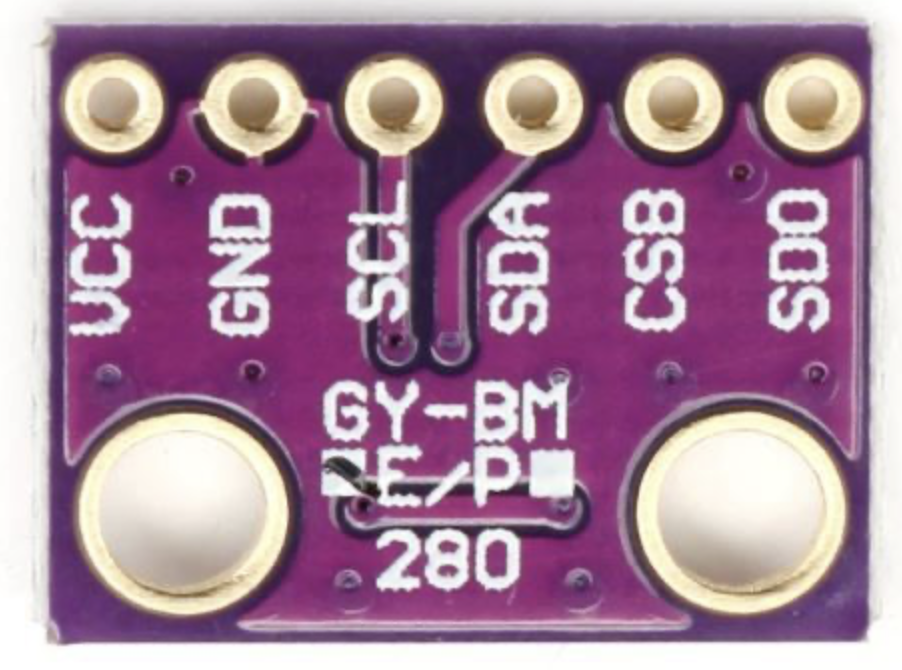
\includegraphics[width=\linewidth]{bme280.png}
    \caption{BME280}
    \label{fig:smalldiagram}
\end{figure}
\begin{figure}[ht!]
    \centering
    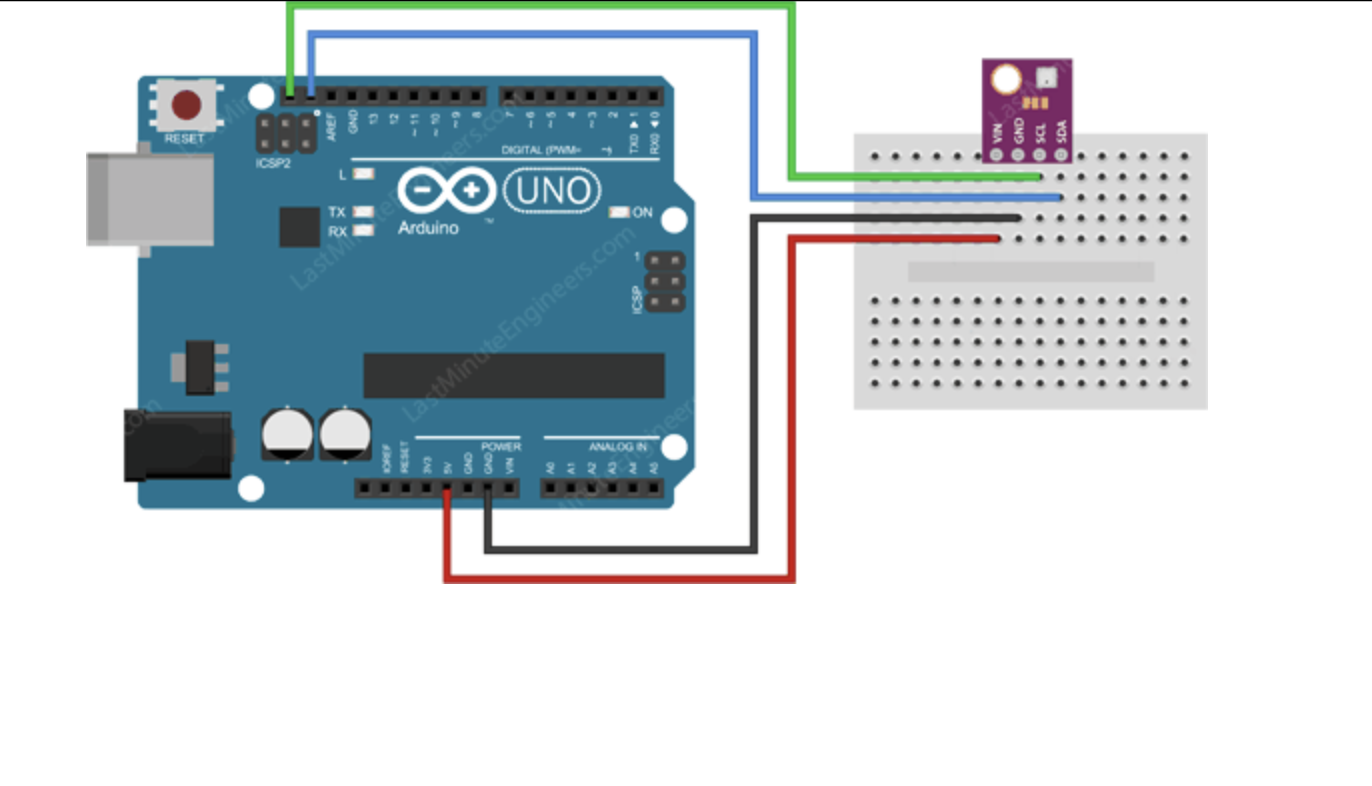
\includegraphics[width=\linewidth]{bme280_wiring.png}
    \caption{BME280 wiring}
    \label{fig:smalldiagram}
\end{figure}
For WAN communication, SIM800L module is used.
\begin{figure}[ht!]
    \centering
    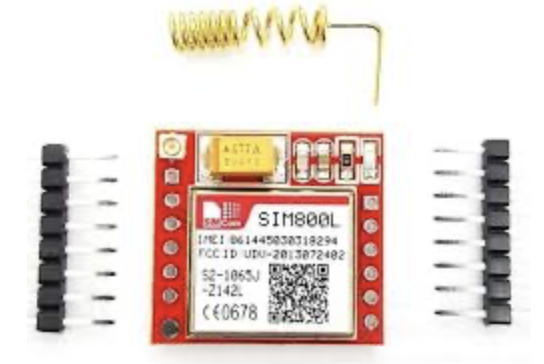
\includegraphics[width=\linewidth]{sim800l.png}
    \caption{SIM800L Module}
    \label{fig:smalldiagram}
\end{figure}
\begin{figure}[ht!]
    \centering
    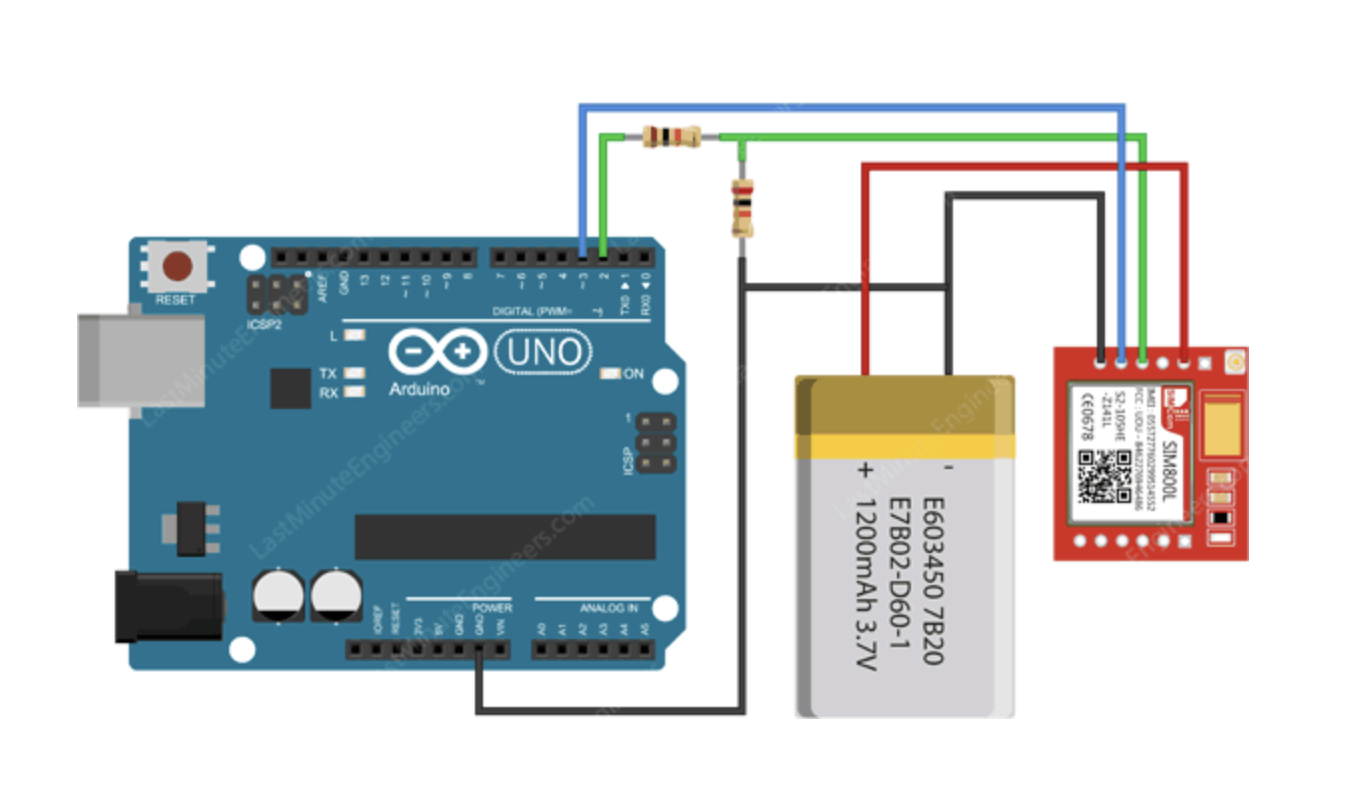
\includegraphics[width=\linewidth]{sim800l_wiring.png}
    \caption{System architecture}
    \label{fig:smalldiagram}
\end{figure}
For lab integration tests, Arduino UNO is used.\\
\begin{figure}[ht!]
    \centering
    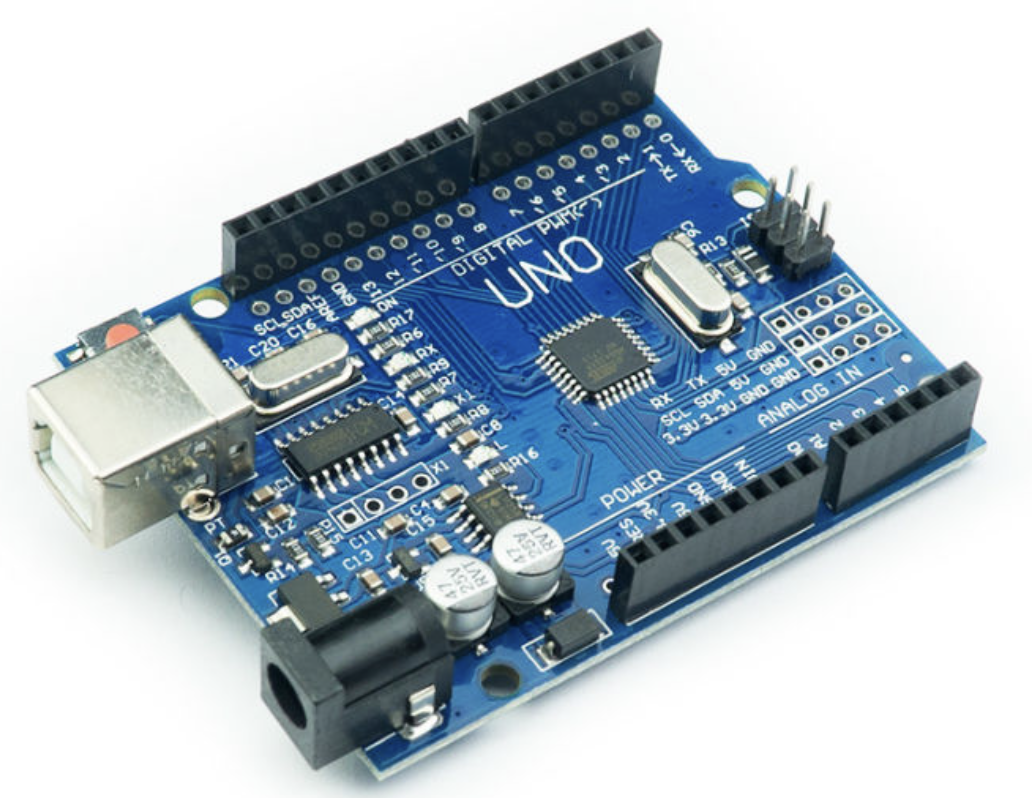
\includegraphics[width=\linewidth]{uno.png}
    \caption{Arduino UNO}
    \label{fig:smalldiagram}
\end{figure}
For driving valve, a 9V latched valve and L298N driver is used.
\begin{figure}[ht!]
    \centering
    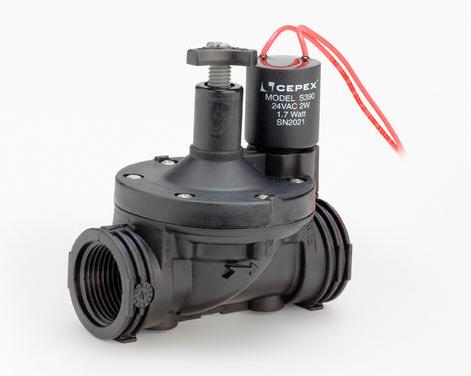
\includegraphics[width=\linewidth]{valve.jpeg}
    \caption{Valve}
    \label{fig:smalldiagram}
\end{figure}
\begin{figure}[ht!]
    \centering
    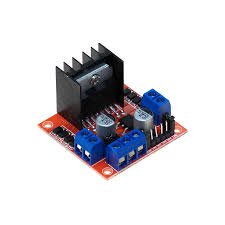
\includegraphics[width=\linewidth]{l298n.jpeg}
    \caption{L298N}
    \label{fig:smalldiagram}
\end{figure}
\subsection{Performance Results}
% Present the main results obtained from your implementation, simulation, experiment, or
% optimization study.
% Depending on your project, this may include:
% \begin{itemize}
% \item execution time, latency, throughput, or response time,
% \item energy or power consumption,
% \item memory usage or resource utilization,
% \item accuracy, error rate, detection rate, or other quality metrics,
% \item optimization objective values,
% \item comparison of different parameter settings,
% \item screenshots or outputs demonstrating that the system works.
% \end{itemize}
% Clearly explain the experimental setup and the meaning of each result.
As full integration is not achieved, separate performances of the components will be evaluated.\\
SIM800L is a cheap module for cellular network usage. It provides message and audio communication interfaces. Nevertheless, the module doesn't have any electrical protection, so even though one-time voltage just 0.1 V above the limit damages it. Also as it's native antenna has very little power, a seperate antenna is needed, which increases costs.\\
BME280 is one of the most widely used environmental measurement sensor. It is very easy to use and provides SPI and I2C interfaces for the user.\\
Arduino Uno is one of the most user-friendly and well-documented boards in the market. It is very easy to integrate sensors to it. Serial monitor provided by Arduino IDE is also very useful debugging tool.\\
For valve control, a 9V DC latched valve and a L298N driver (H-bridge) is used. It's been observed that after changing the polarity of valve and there the position, no power is used.
\subsection{Comparative Analysis}
Not applicable.
\subsection{Discussion}
Throughout the project, following problems and observations are made:
\begin{itemize}
    \item Generally, chosen sensors and components are observed to be low quality and have lot-to-lot malfunctions. Also they are really prone to small errors in power supply, they can easily burn.
    \item Main achievement of the project was to observe that more quality components should be chosen as the ones used can easily malfunction and in real system as reaching and repairing them will not be easy.
    \item Current methodology didn't suppress any limitations in lab integration tests, but at full system integration problem of malfunctioning components is expected as conditions are hard. Also possible problems for WAN and LAN communications are still there as they are not expexted at real environment.
    \item Reliability of components had a huge effect on project, as it lead time loss in debugging. Also using cheap power supplies caused many problems.
\end{itemize}
% Critically discuss your results.
% You should address questions such as:
% \begin{itemize}
% \item What worked as expected? \\
% Sensors are low quality
% \item What did not work as expected?
% \item What are the main achievements of your project?
% \item What are the limitations of your current implementation or methodology?
% \item What trade-offs did you observe?
% \item Were there any unexpected results?
% \item How do embedded system design concerns such as real-time behavior, energy
% efficiency, reliability, safety/security, or resource constraints affect your
% results?
% \end{itemize}
\subsection{Reproducibility}
% Describe how your work can be reproduced by another researcher or student.
% Include relevant details such as:
% \begin{itemize}
% \item code availability, including repository link if the code can be shared,
% \item programming language, libraries, tools, simulators, frameworks, or hardware
% platforms used,
% \item operating system and environment details,
% \item configuration files or important implementation settings,
% \item parameter values used in experiments or optimization,
% \item dataset name, source, access link, or data generation method,
% \item instructions for running the code or reproducing the experiments.
% \end{itemize}
% The goal is to make your work understandable and repeatable.
Easiest way to reproduce the work is as the following:
\begin{itemize}
    \item Download Arduino IDE
    \item Make the wirings as given
    \item For each component, upload the code given in repository and observe the result via serial monitor
\end{itemize}
\section{Conclusion and Future Work}
% Summarize the overall project and its final status.
% Your conclusion should include:
% \begin{itemize}
% \item the problem addressed in the project,
% \item the main methodology followed,
% \item the main results and findings,
% \item what was successfully completed,
% \item what could not be completed or did not work as planned,
% \item the main limitations of the current work,
% \item possible improvements or extensions,
% \item future work that could be done after this course project.
% \end{itemize}
% Be honest and specific. A good conclusion should clearly show what was achieved and
% what remains open.\\
As mentioned before, due to time concerns even though components and main code layout are designed and implemented, full system integration was not achieved. So, the final project stage is lab integration tests. Nevertheless, all of the components were purchased and their integration are done to the some level.

\bibliographystyle{IEEEtran}
\bibliography{references}

\end{document}